\chapter{Resultados de Simulação e Experimentais}

\section{Simulação}
Utilizando a Robotics Toolbox \citep{petercorke} para MATLAB, foram feitas simulações para o controle cinemático utilizando controle proporcional com feedforward. 

\begin{gather}
\bm{x_d} = \m{75 \sin(\omega_n t) + \sin (4 \omega_n t) + 500 \\ 57 \\ 75 \cos(\omega_n t) + \cos(4\omega_n t) -67 \\ \omega_n \sin(\omega_nt) }
\qquad
\bm{\dot{x}_d} = \m{75\omega_n \cos(t\omega_n) + 300 \omega_n \cos(4t\omega_n) \\
0 \\
-75 \omega_n \sin(t \omega_n) - 300 \omega_n \sin(4t\omega_n) \\
\omega_n^2 \cos(t \omega_n)}
\end{gather}


\begin{figure}[H]
\centering
  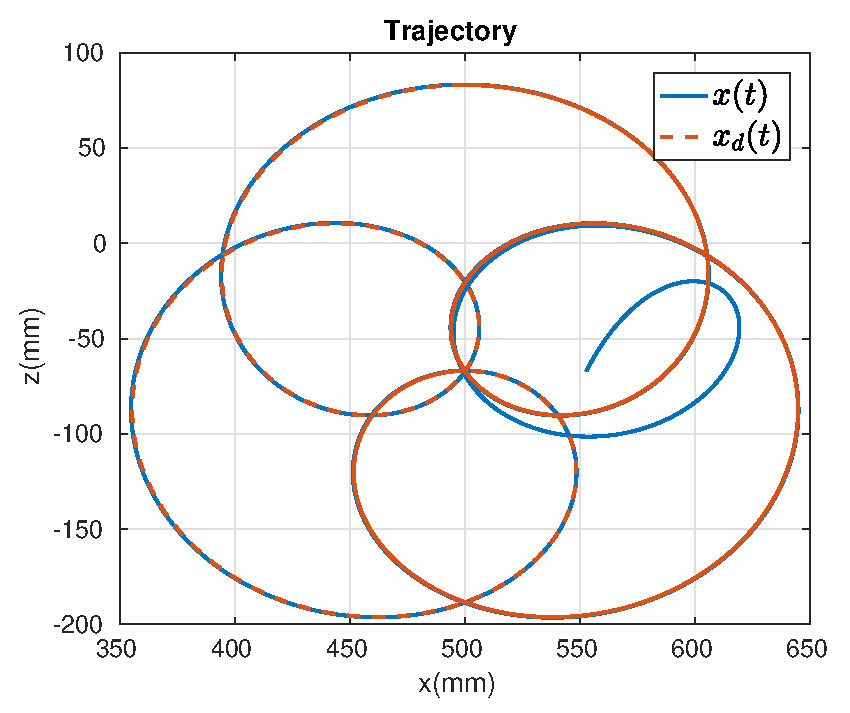
\includegraphics[width=0.5\linewidth]{./img/simul_delay_zoh1/traj.eps}
  \caption{Trajetória 1 no plano x-z}
  \label{fig:sub1}
\end{figure}%

\begin{figure}[H]
\centering
\begin{subfigure}{.5\textwidth}
  \centering
  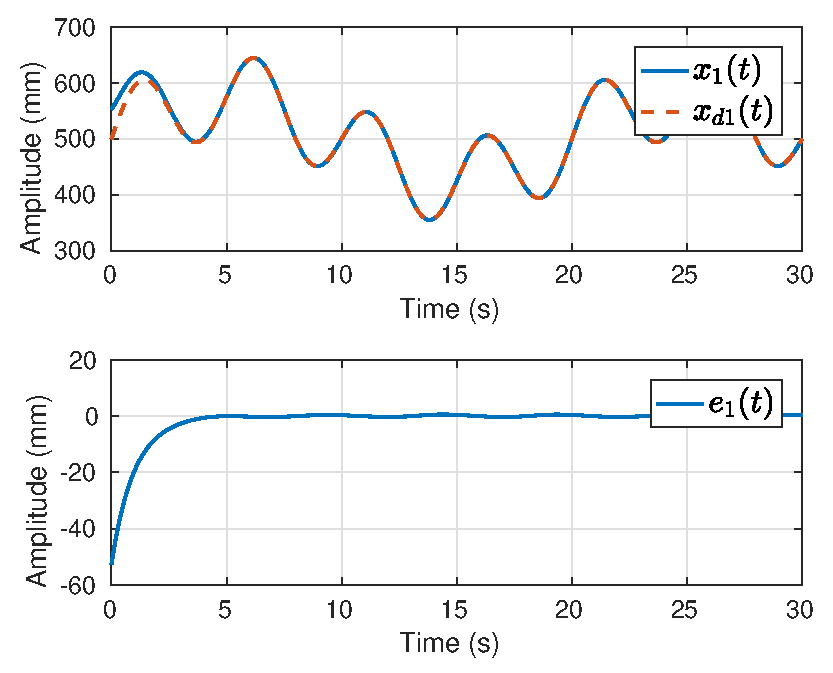
\includegraphics[width=\linewidth]{./img/simul_delay_zoh1/x1.eps}
  \caption{$x_1$, $x_{d1}$ e $e_1$}
  \label{fig:sub1}
\end{subfigure}%
\begin{subfigure}{.5\textwidth}
  \centering
  \includegraphics[width=\linewidth]{./img/simul_delay_zoh1/x2.eps}
  \caption{$x_2$, $x_{d2}$ e $e_2$}
  \label{fig:sub2}
\end{subfigure}
\begin{subfigure}{.5\textwidth}
  \centering
  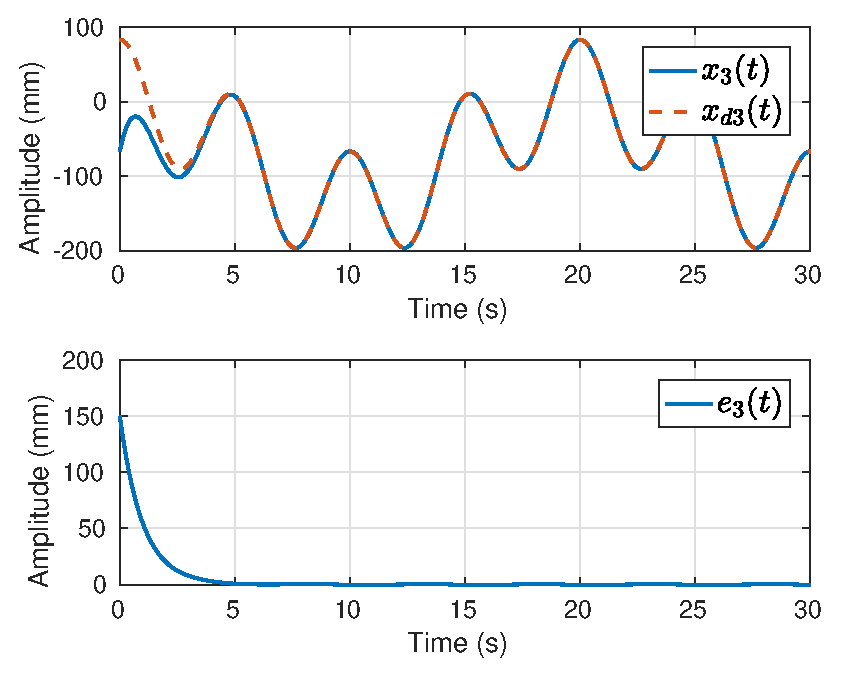
\includegraphics[width=\linewidth]{./img/simul_delay_zoh1/x3.eps}
  \caption{$x_3$, $x_{d3}$ e $e_3$}
  \label{fig:sub1}
\end{subfigure}%
\begin{subfigure}{.5\textwidth}
  \centering
  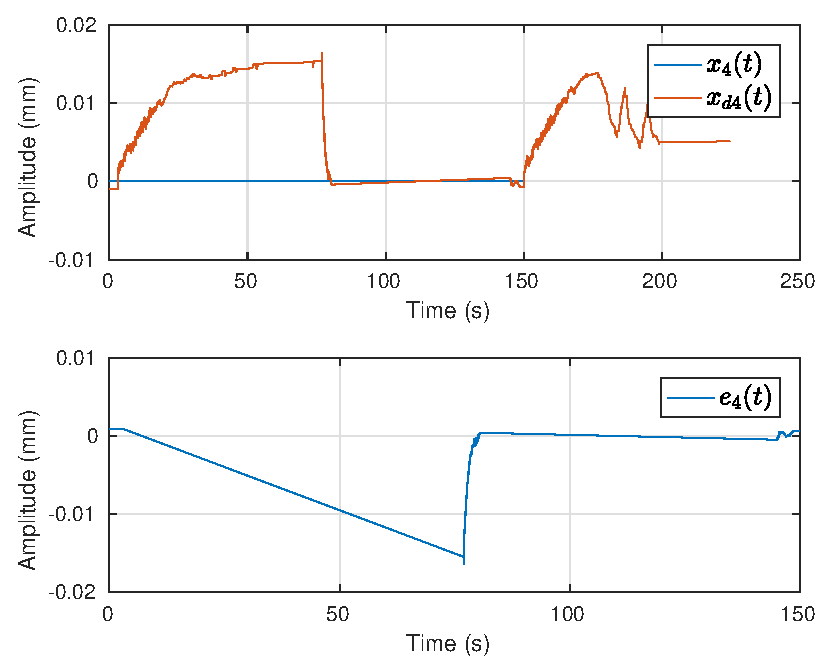
\includegraphics[width=\linewidth]{./img/simul_delay_zoh1/x4.eps}
  \caption{$x_4$, $x_{d4}$ e $e_4$}
  \label{fig:sub2}
\end{subfigure}
\caption{Rastreamento da trajetória 1 para $\bm{K}_t = \bm{I}$}
\label{fig:test}
\end{figure}

\begin{figure}[H]
\centering
\begin{subfigure}{.5\textwidth}
  \centering
  \includegraphics[width=\linewidth]{./img/simul_delay_zoh1/error.eps}
  \caption{$e_1$ e $e_3$}
  \label{fig:sub1}
\end{subfigure}%
\begin{subfigure}{.5\textwidth}
  \centering
  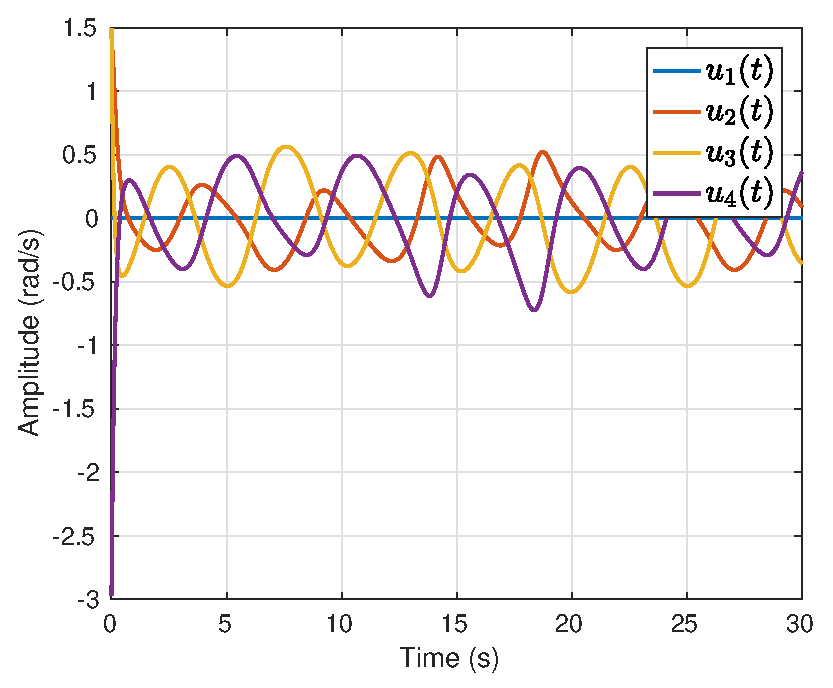
\includegraphics[width=\linewidth]{./img/simul_delay_zoh1/u.eps}
  \caption{$\bm{u}(t)$}
  \label{fig:sub2}
\end{subfigure}
\caption{Trajetória 1: Destaque para o erro $e_1$ e $e_3$ com $\bm{K}_t = \bm{I}$}
\label{fig:erro_traj}
\end{figure}


\section{Análise da Malha de Controle a nível de Juntas}
Para verificar se de fato são válidas as premissas assumidas na seção \ref{sec:controle_cinematico}para aplicação de uma estratégia de controle cinemático foi levantada para cada uma das juntas a resposta a uma onda quadrada tal que:
\[ u = A \sgn(\sin( 2\pi t/f)) \]
onde o período $T = 1/f = 1s$ e a amplitude $A = 0.5 rad/s$

\newlength{\imageheight}
\begin{figure}[H]
  \centering
  	\settoheight{\imageheight}{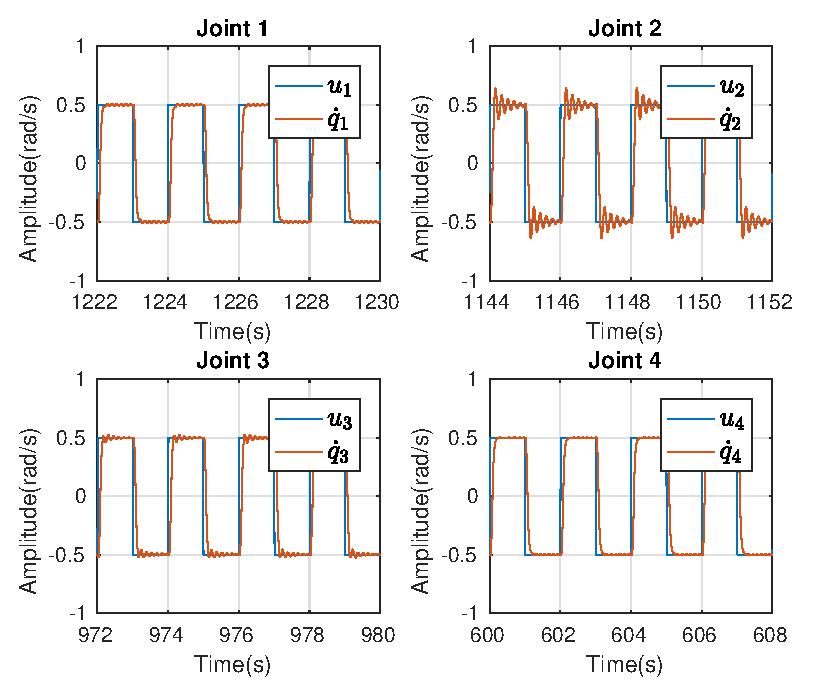
\includegraphics{./img/internal_loop}}
    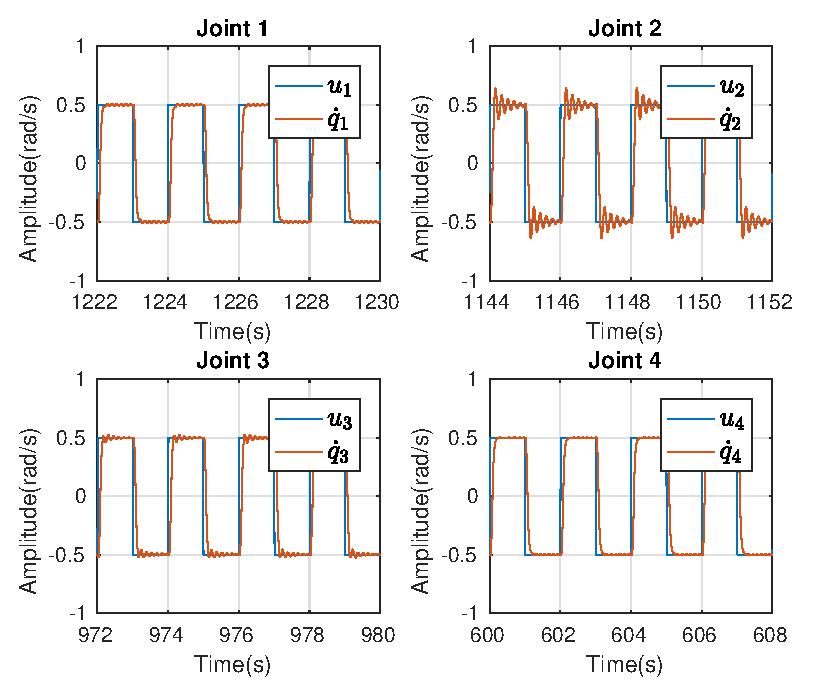
\includegraphics[width=\textwidth, clip=true, trim = 0 0.5\imageheight 0 0 0 mm]{./img/internal_loop}
  \caption{Resposta de velocidade das juntas 1 e 2}
\end{figure}

\begin{figure}[H]
  \centering
  	\settoheight{\imageheight}{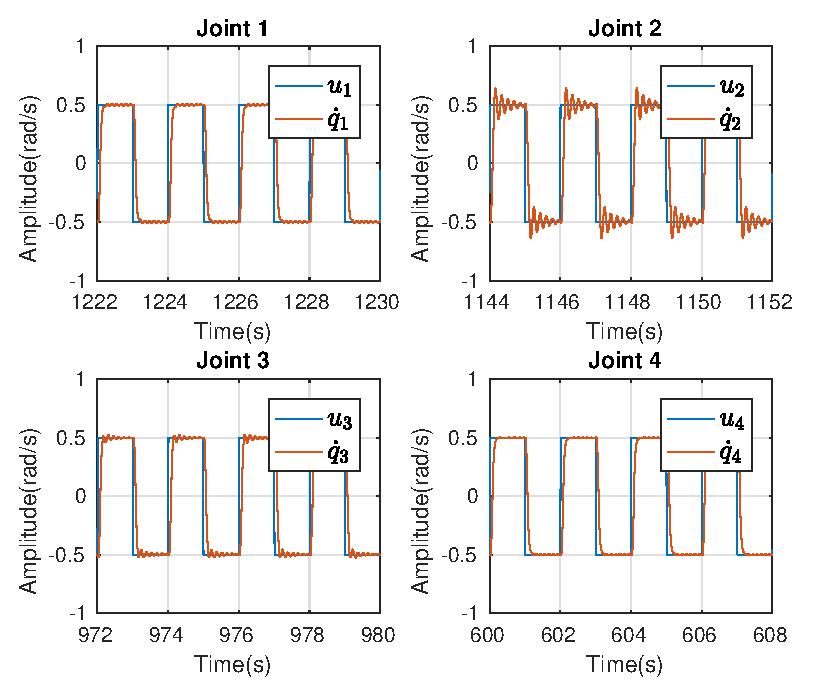
\includegraphics{./img/internal_loop}}
    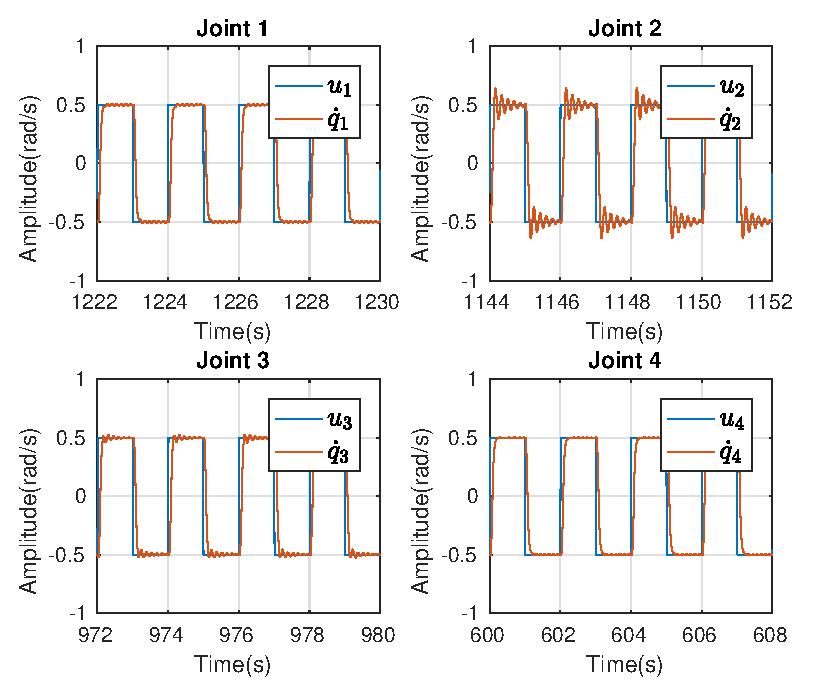
\includegraphics[width=\textwidth, clip=true, trim = 0 0 0 0.5\imageheight 0 mm]{./img/internal_loop}
  \caption{Resposta de velocidade das juntas 3 e 4}
\end{figure}


Observa-se que para as juntas 1, 3 e 4 a resposta é de primeira ordem, enquanto que para a junta 2 observa-se que existe uma dinâmica.
	

\section{Controle de Posição no Espaço das Juntas}

Neste experimento foi testado controle de posição no espaço das juntas, partindo da posição $\bm{q} =[ 0 \;\; -\pi/2 \;\; 0 \;\; 0]^T$, deseja-se atingir a posição $\bm{q} =[ 0 \;\; -\pi/4 \;\; \pi/2  \;\; -\pi/4]^T$
\begin{figure}[H]
\centering
\begin{subfigure}{.5\textwidth}
  \centering
  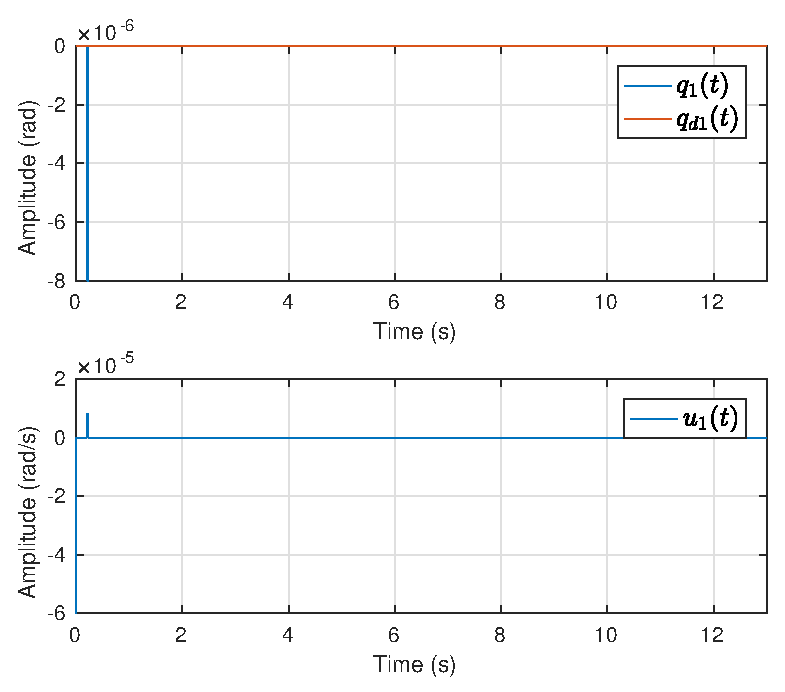
\includegraphics[width=\linewidth]{./img/joint_test1/q1.eps}
  \caption{Junta 1}
  \label{fig:sub1}
\end{subfigure}%
\begin{subfigure}{.5\textwidth}
  \centering
  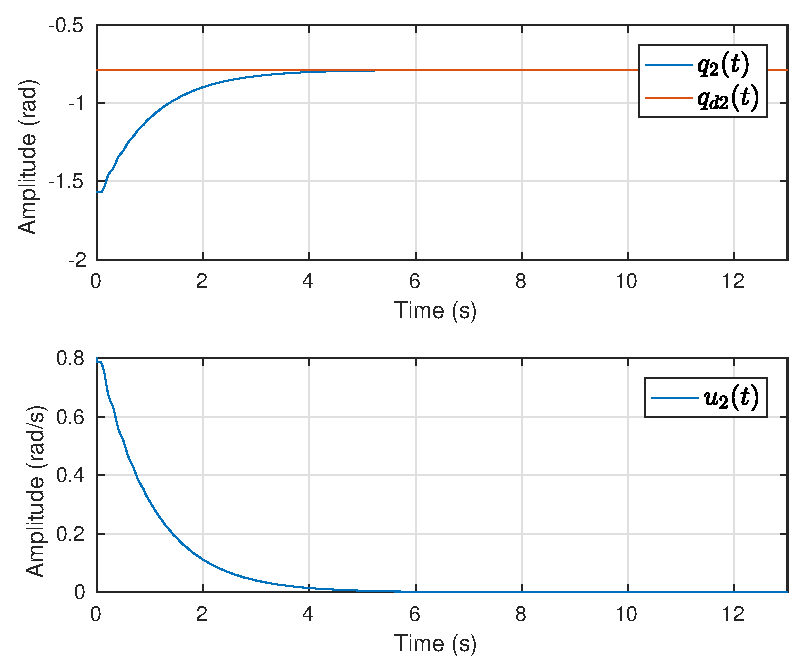
\includegraphics[width=\linewidth]{./img/joint_test1/q2.eps}
  \caption{Junta 2}
  \label{fig:sub2}
\end{subfigure}
\begin{subfigure}{.5\textwidth}
  \centering
  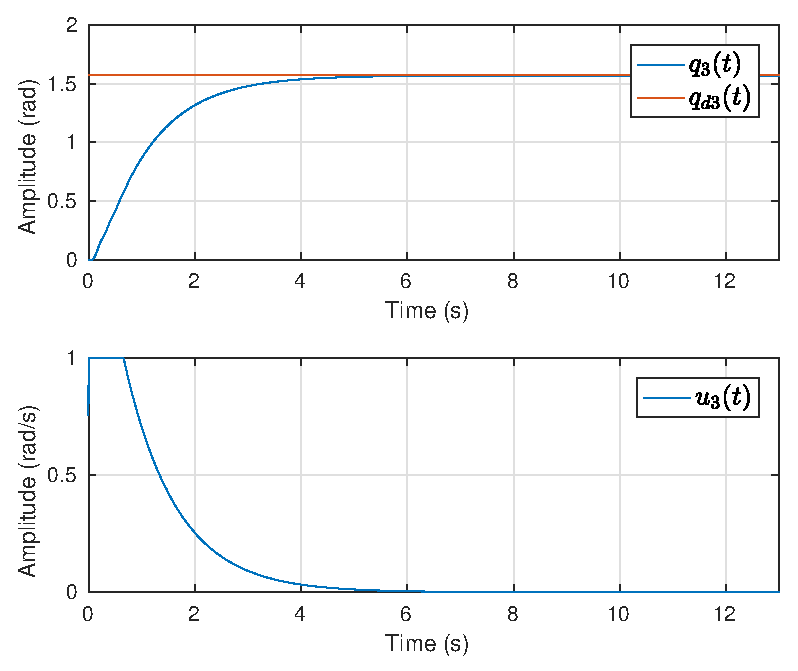
\includegraphics[width=\linewidth]{./img/joint_test1/q3.eps}
  \caption{Junta 3}
  \label{fig:sub1}
\end{subfigure}%
\begin{subfigure}{.5\textwidth}
  \centering
  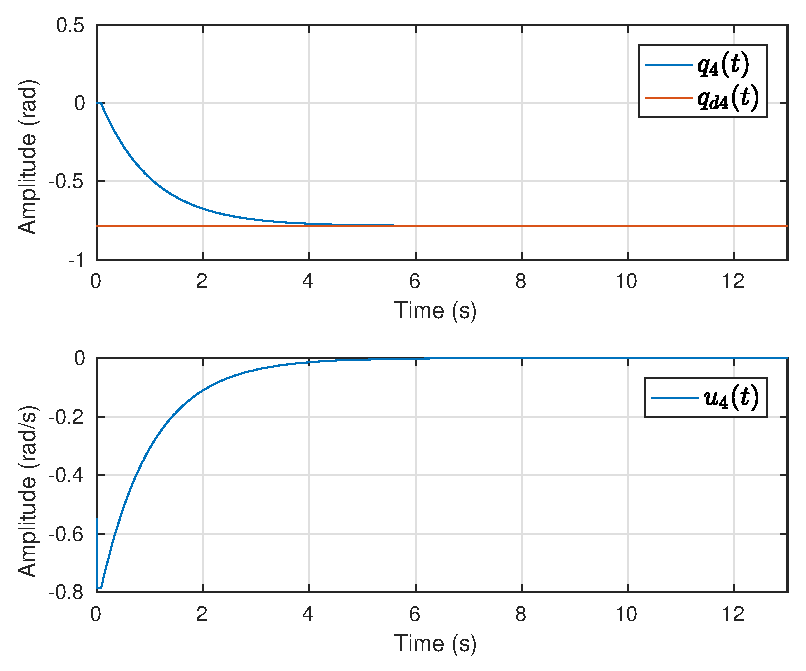
\includegraphics[width=\linewidth]{./img/joint_test1/q4.eps}
  \caption{Junta 4}
  \label{fig:sub2}
\end{subfigure}
\caption{Controle de Posição no Espaço das Juntas}
\label{fig:test}
\end{figure}


\section{Controle de Posição no Espaço Operacional}

\subsection{Experimento 1}

\begin{figure}[H]
\centering
\begin{subfigure}{.5\textwidth}
  \centering
  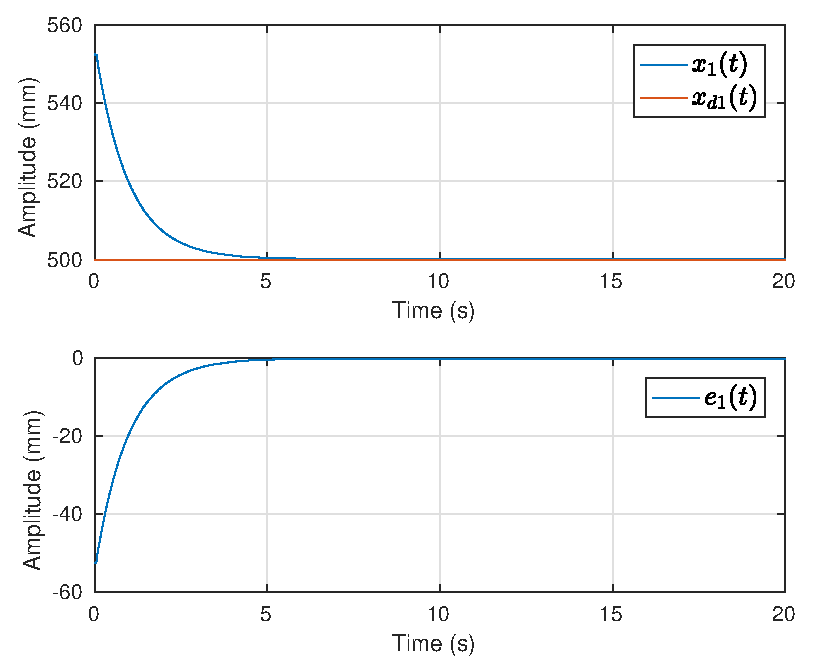
\includegraphics[width=\linewidth]{./img/position1/x1.eps}
  \caption{$x$}
  \label{fig:sub1}
\end{subfigure}%
\begin{subfigure}{.5\textwidth}
  \centering
  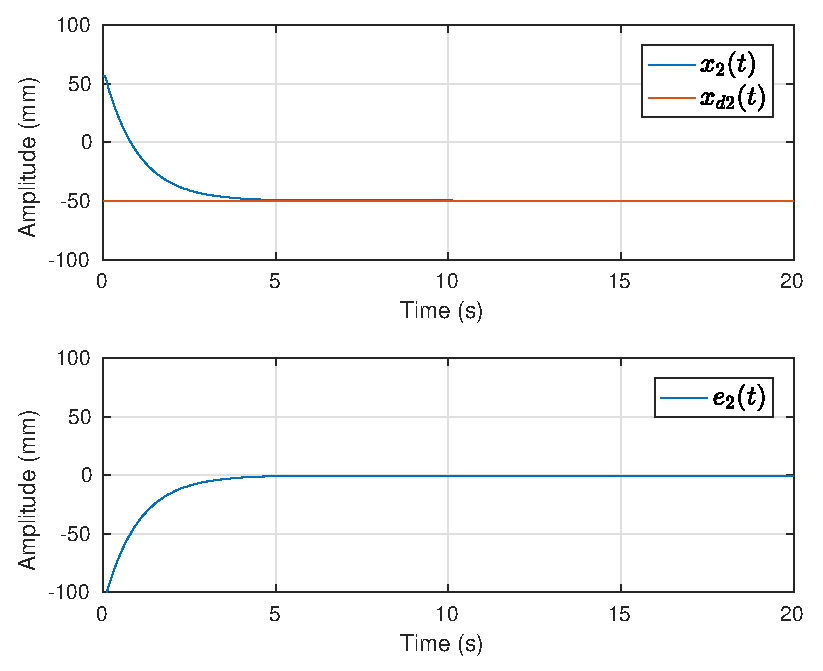
\includegraphics[width=\linewidth]{./img/position1/x2.eps}
  \caption{$y$}
  \label{fig:sub2}
\end{subfigure}
\begin{subfigure}{.5\textwidth}
  \centering
  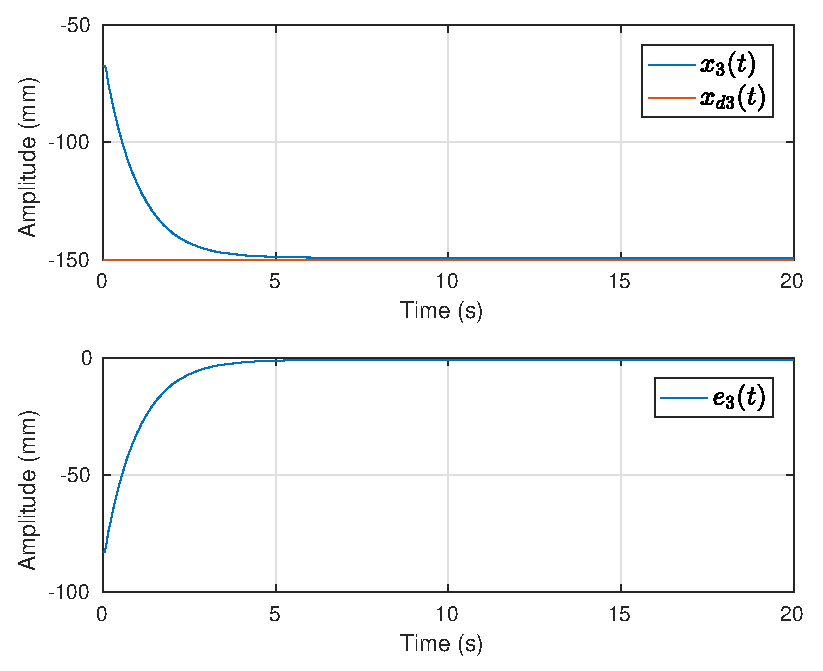
\includegraphics[width=\linewidth]{./img/position1/x3.eps}
  \caption{$z$}
  \label{fig:sub1}
\end{subfigure}%
\begin{subfigure}{.5\textwidth}
  \centering
  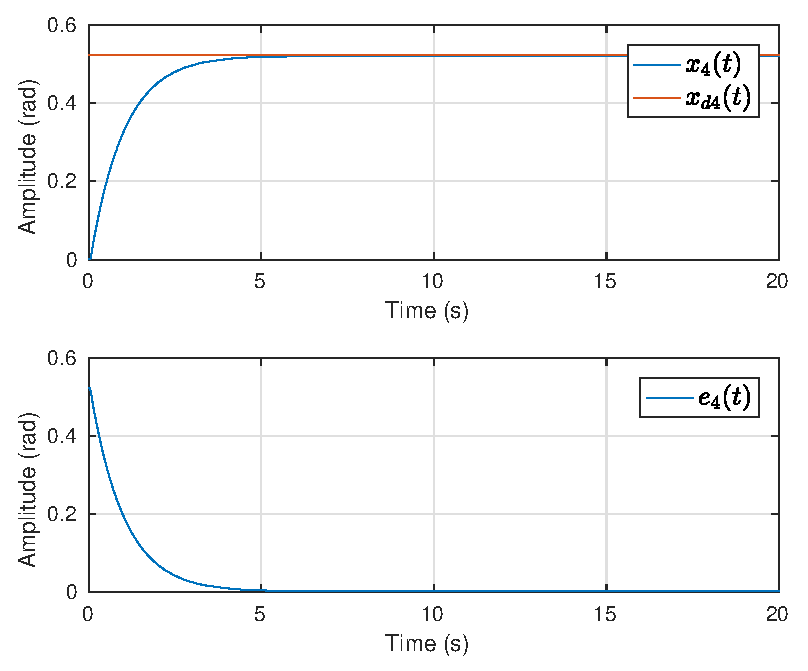
\includegraphics[width=\linewidth]{./img/position1/x4.eps}
  \caption{$\phi$}
  \label{fig:sub2}
\end{subfigure}
\caption{Controle de Posição no Espaço Operacional}
\label{fig:test}
\end{figure}

\subsection{Experimento 2}

Neste experimento, demonstra-se o controle no espaço operacional.
A posição inicial é $\bm{x} =[ 550 \; 57 \; -100 \; 0]^T$. O gráfico \ref{fig:pos_exp2_phi} a orientação é alterada para $60^o$, ou seja $\bm{x_d} =[ 550 \; 57 \; -100 \; 1.0472]^T$. Em seguida, a orientação é alterada para $-60^o$, ou seja $\bm{x_d} =[ 550 \; 57 \; -100 \; -1.0472]^T$. 

\begin{figure}[H]
\centering
\begin{subfigure}{.5\textwidth}
  \centering
  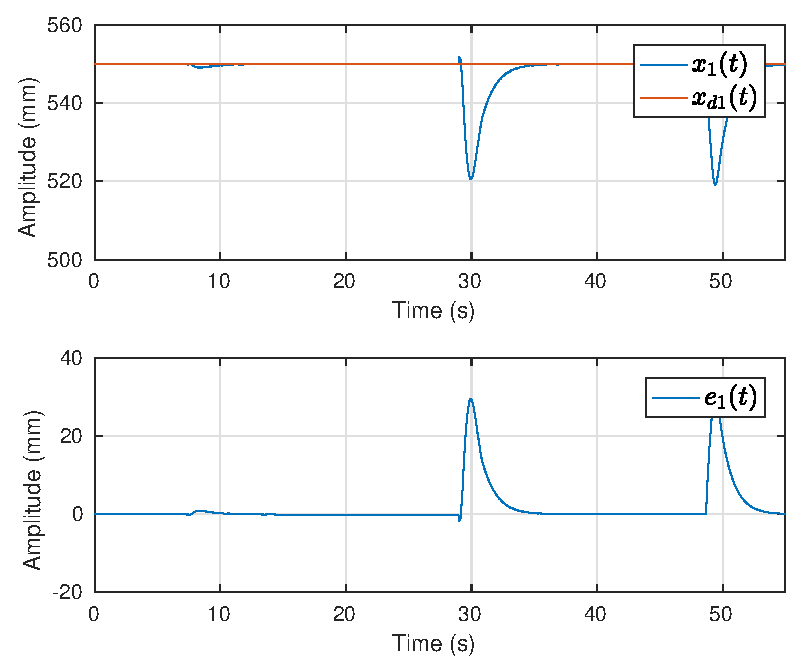
\includegraphics[width=\linewidth]{./img/position2/x1.eps}
  \caption{$x$}
  \label{fig:sub1}
\end{subfigure}%
\begin{subfigure}{.5\textwidth}
  \centering
  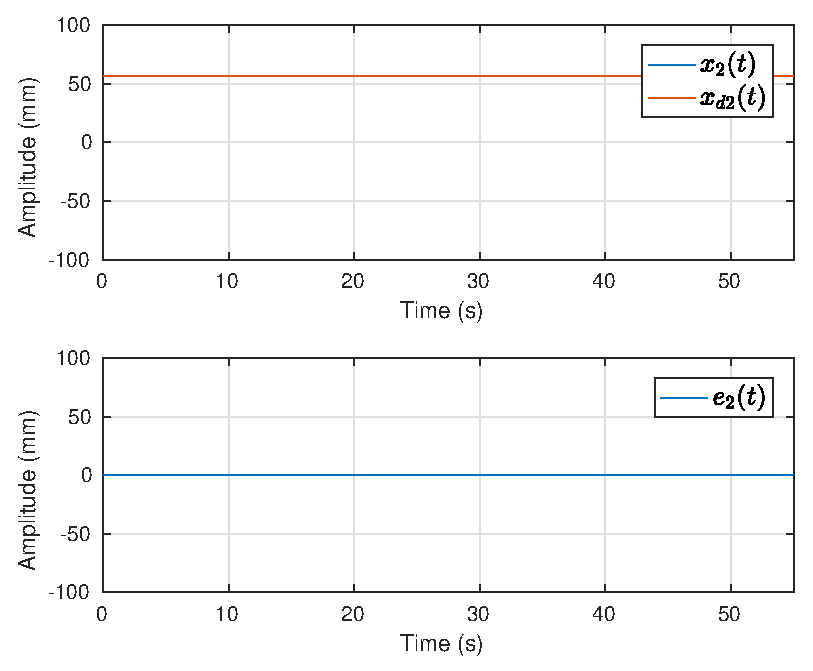
\includegraphics[width=\linewidth]{./img/position2/x2.eps}
  \caption{$y$}
  \label{fig:sub2}
\end{subfigure}
\begin{subfigure}{.5\textwidth}
  \centering
  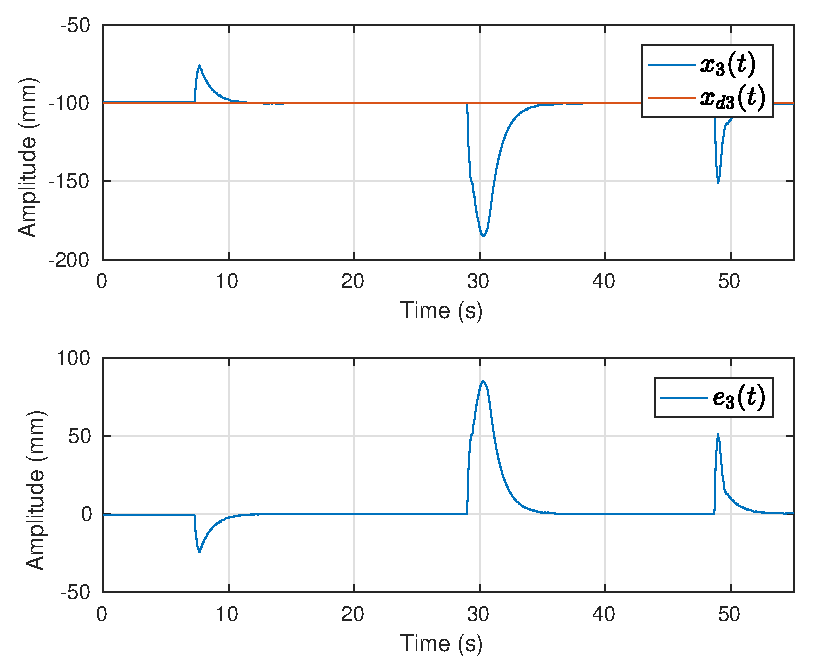
\includegraphics[width=\linewidth]{./img/position2/x3.eps}
  \caption{$z$}
  \label{fig:sub1}
\end{subfigure}%
\begin{subfigure}{.5\textwidth}
  \centering
  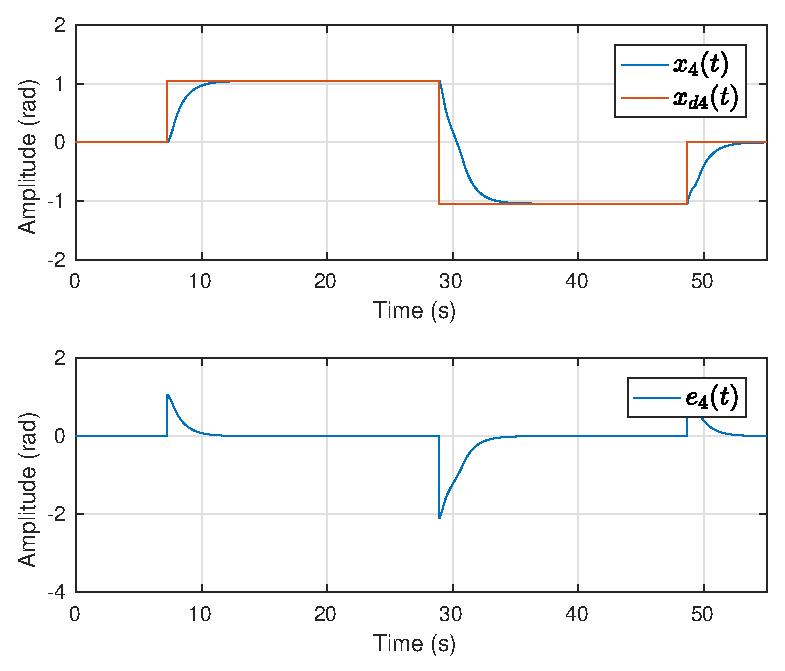
\includegraphics[width=\linewidth]{./img/position2/x4.eps}
  \caption{$\phi$}
  \label{fig:pos_exp2_phi}
\end{subfigure}
\caption{Controle de Posição no Espaço Operacional}
\label{fig:test}
\end{figure}

\section{Rastreamento de Trajetória}

\subsection{Trajetória 1}
A trajetória a ser rastreada é dada pelas equações:
\begin{gather}
\bm{x_d} = \m{75 \sin(\omega_n t) + \sin (4 \omega_n t) + 500 \\ 57 \\ 75 \cos(\omega_n t) + \cos(4\omega_n t) -67 \\ \omega_n \sin(\omega_nt) }
\qquad
\bm{\dot{x}_d} = \m{75\omega_n \cos(t\omega_n) + 300 \omega_n \cos(4t\omega_n) \\
0 \\
-75 \omega_n \sin(t \omega_n) - 300 \omega_n \sin(4t\omega_n) \\
\omega_n^2 \cos(t \omega_n)}
\end{gather}

Onde $\omega_n = \pi/10$

\subsubsection{Ganho $\bm{K}_t = \bm{I}$}

\begin{figure}[H]
\centering
  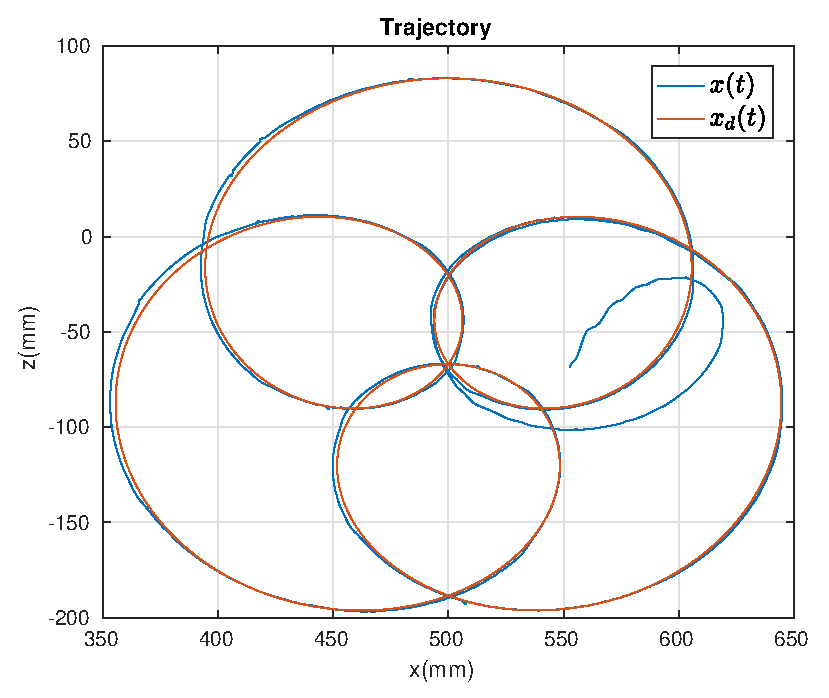
\includegraphics[width=0.5\linewidth]{./img/traj_1_k1/traj.eps}
  \caption{Trajetória 1 no plano x-z}
  \label{fig:sub1}
\end{figure}%

\begin{figure}[H]
\centering
\begin{subfigure}{.5\textwidth}
  \centering
  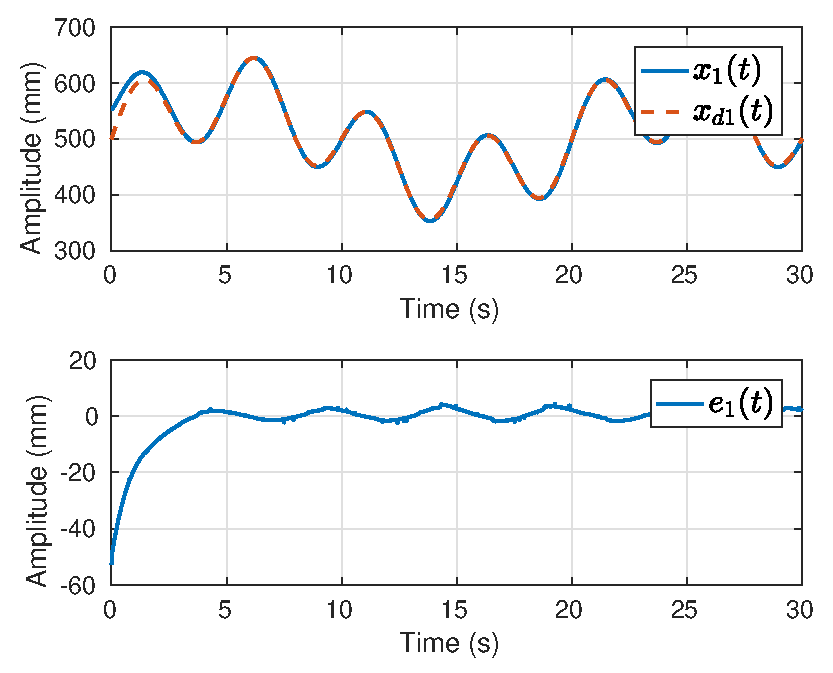
\includegraphics[width=\linewidth]{./img/traj_1_k1/x1.eps}
  \caption{$x_1$, $x_{d1}$ e $e_1$}
  \label{fig:sub1}
\end{subfigure}%
\begin{subfigure}{.5\textwidth}
  \centering
  \includegraphics[width=\linewidth]{./img/traj_1_k1/x2.eps}
  \caption{$x_2$, $x_{d2}$ e $e_2$}
  \label{fig:sub2}
\end{subfigure}
\begin{subfigure}{.5\textwidth}
  \centering
  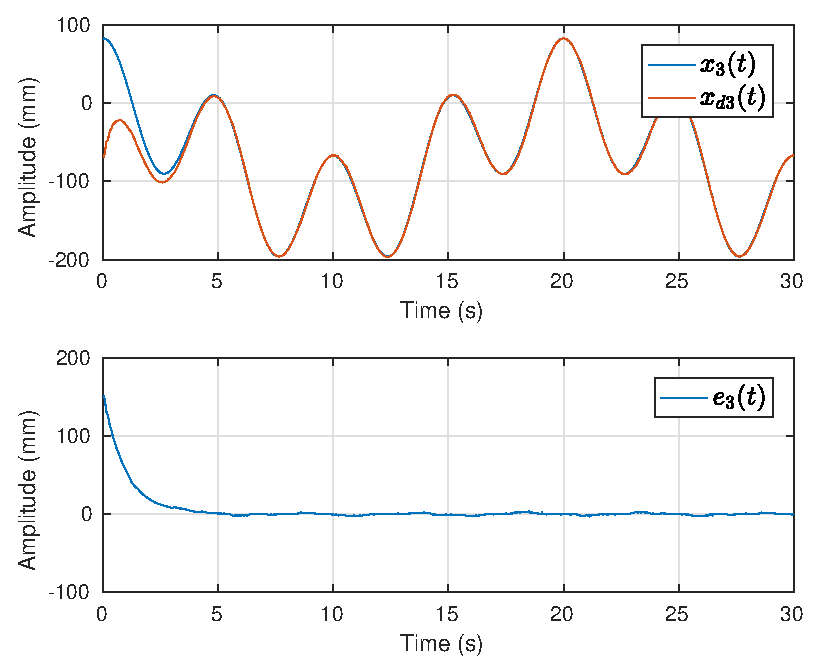
\includegraphics[width=\linewidth]{./img/traj_1_k1/x3.eps}
  \caption{$x_3$, $x_{d3}$ e $e_3$}
  \label{fig:sub1}
\end{subfigure}%
\begin{subfigure}{.5\textwidth}
  \centering
  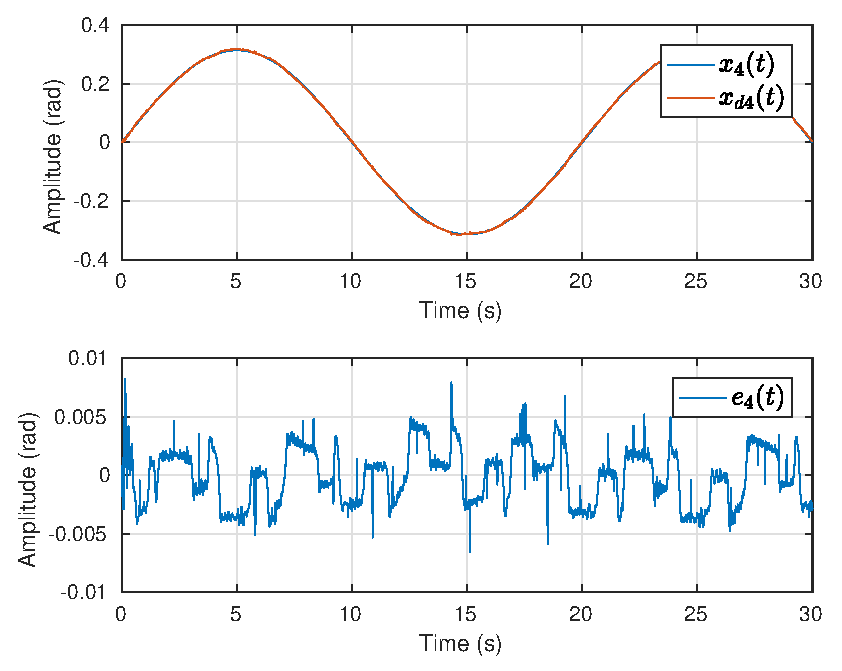
\includegraphics[width=\linewidth]{./img/traj_1_k1/x4.eps}
  \caption{$x_4$, $x_{d4}$ e $e_4$}
  \label{fig:sub2}
\end{subfigure}
\caption{Rastreamento da trajetória 1 para $\bm{K}_t = \bm{I}$}
\label{fig:test}
\end{figure}

\begin{figure}[H]
\centering
\begin{subfigure}{.5\textwidth}
  \centering
  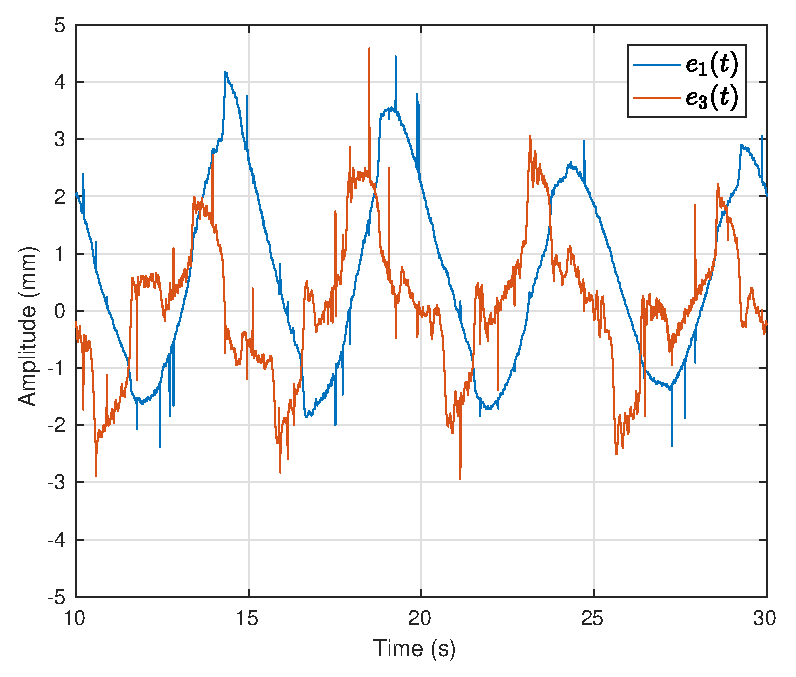
\includegraphics[width=\linewidth]{./img/traj_1_k1/error.eps}
  \caption{$e_1$ e $e_3$}
  \label{fig:sub1}
\end{subfigure}%
\begin{subfigure}{.5\textwidth}
  \centering
  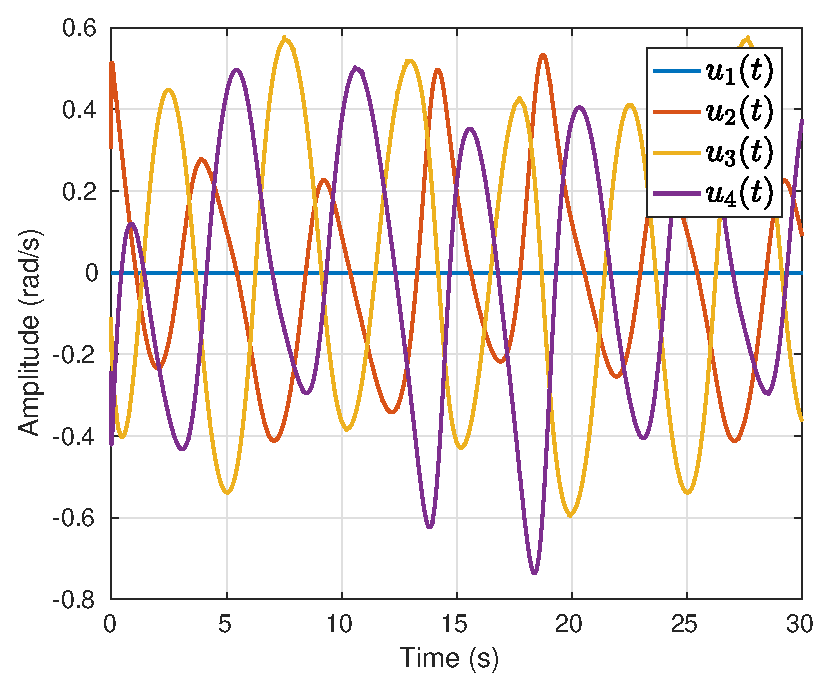
\includegraphics[width=\linewidth]{./img/traj_1_k1/u.eps}
  \caption{$\bm{u}(t)$}
  \label{fig:sub2}
\end{subfigure}
\caption{Trajetória 1: Destaque para o erro $e_1$ e $e_3$ com $\bm{K}_t = \bm{I}$}
\label{fig:erro_traj}
\end{figure}

Podem-se observar diversos picos no gráfico do erro na figura \ref{fig:erro_traj} que se devem ao fato de, por não se tratar de um sistema em tempo-real, o período de controle pode sofrer variação caso aconteça alguma interrupção no sistema operacional. Assim, o comando não seria atualizado, resultando em um erro maior na próxima iteração.


\subsection{Trajetória 2}
A trajetória a ser rastreada é dada pelas equações:


\begin{align}
\bm{x_d} &= \m{ 
\ddfrac{100 \cos(t)}{\sin^2(t) + 1} + 500 \\
57 \\
\ddfrac{100\cos(t) \sin(t)}{\sin^2(t) + 1} -50 \\
0
}^T  &&
\bm{\dot{x}_d} &= \m{
\ddfrac{100\sin(t) (\sin^2(t) -3 )}{(\sin^2(t) + 1)^2} \\
0 \\
\ddfrac{-(300 \sin^2(t) - 100)}{(\sin^2(t) + 1)^2} \\
0}^T
\end{align}

\subsubsection{Ganho $\bm{K}_t = \bm{I}$}
\begin{figure}[H]
\centering
  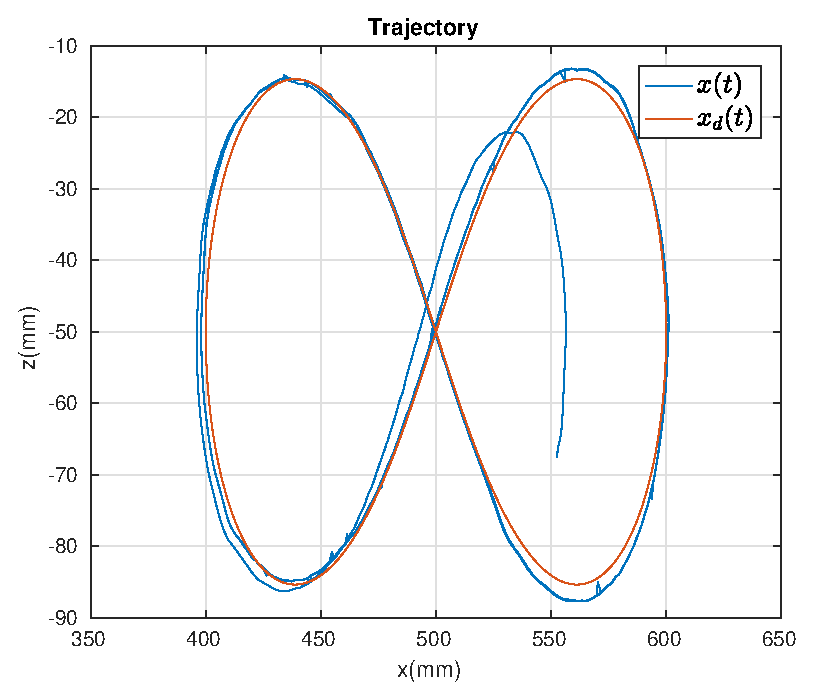
\includegraphics[width=0.5\linewidth]{./img/traj_2_k1/traj.eps}
  \caption{Trajetória 2 no plano x-z}
  \label{fig:sub1}
\end{figure}%

\begin{figure}[H]
\centering
\begin{subfigure}{.5\textwidth}
  \centering
  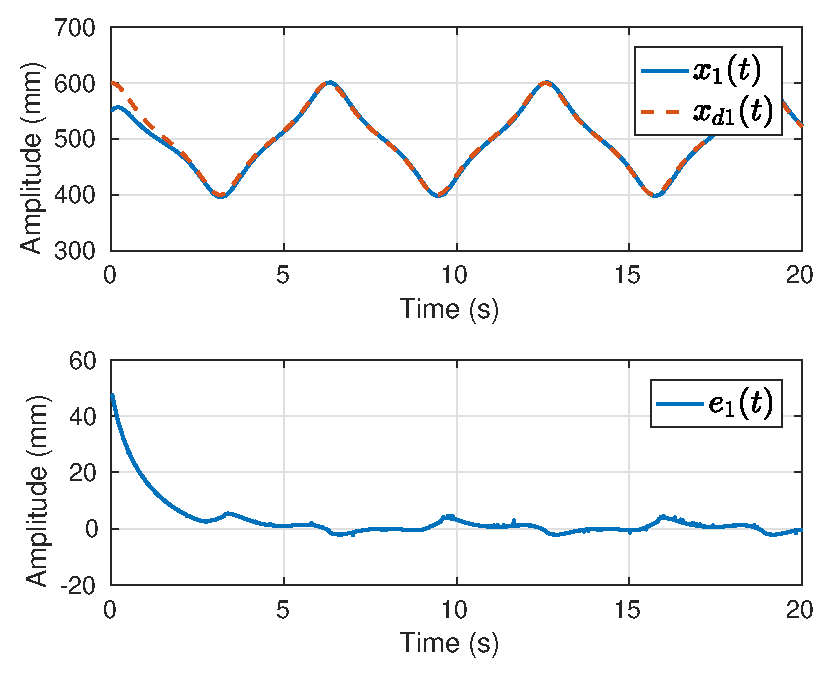
\includegraphics[width=\linewidth]{./img/traj_2_k1/x1.eps}
  \caption{$x_1$, $x_{d1}$ e $e_1$}
  \label{fig:sub1}
\end{subfigure}%
\begin{subfigure}{.5\textwidth}
  \centering
  \includegraphics[width=\linewidth]{./img/traj_2_k1/x2.eps}
  \caption{$x_2$, $x_{d2}$ e $e_2$}
  \label{fig:sub2}
\end{subfigure}
\begin{subfigure}{.5\textwidth}
  \centering
  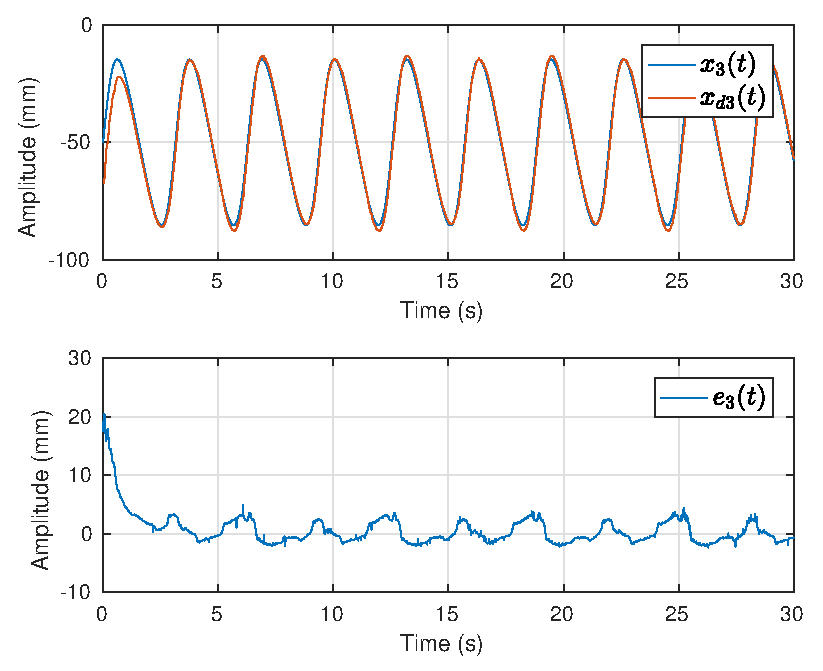
\includegraphics[width=\linewidth]{./img/traj_2_k1/x3.eps}
  \caption{$x_3$, $x_{d3}$ e $e_3$}
  \label{fig:sub1}
\end{subfigure}%
\begin{subfigure}{.5\textwidth}
  \centering
  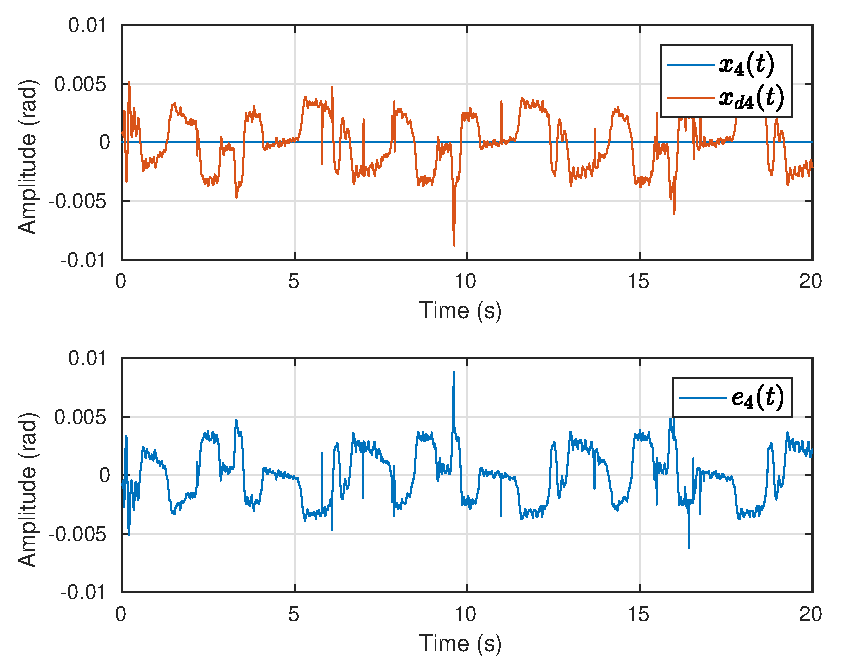
\includegraphics[width=\linewidth]{./img/traj_2_k1/x4.eps}
  \caption{$x_4$, $x_{d4}$ e $e_4$}
  \label{fig:sub2}
\end{subfigure}
\caption{Rastreamento da trajetória 2 para $\bm{K}_t = \bm{I}$}
\label{fig:test}
\end{figure}

\begin{figure}[H]
\centering
\begin{subfigure}{.5\textwidth}
  \centering
  \includegraphics[width=\linewidth]{./img/traj_2_k1/error.eps}
  \caption{$e_1$}
  \label{fig:sub1}
\end{subfigure}%
\begin{subfigure}{.5\textwidth}
  \centering
  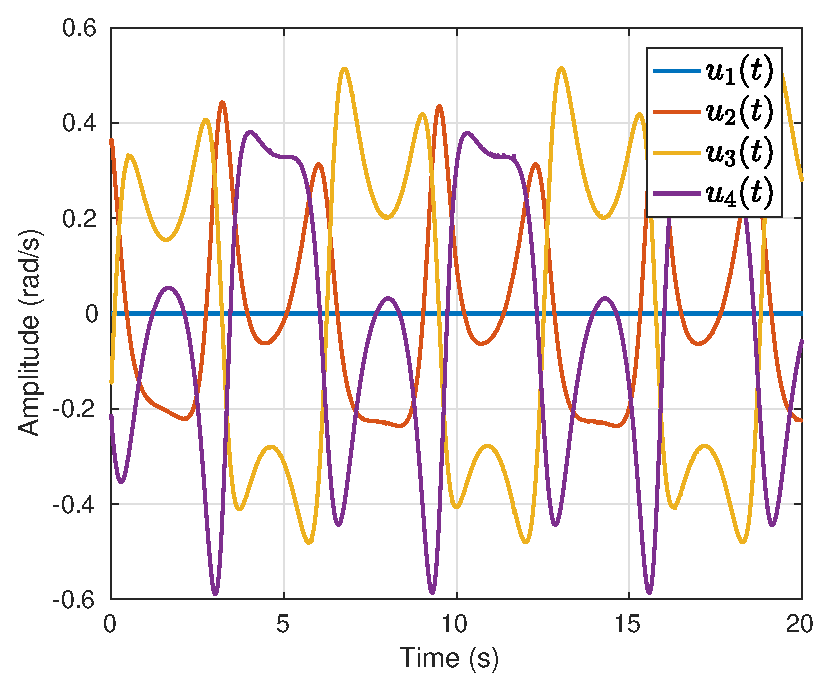
\includegraphics[width=\linewidth]{./img/traj_2_k1/u.eps}
  \caption{$e_3$}
  \label{fig:sub2}
\end{subfigure}
\caption{Trajetória 2: Destaque para o erro $e_1$ e $e_3$ com $\bm{K}_t = \bm{I}$}
\label{fig:erro_traj}
\end{figure}

\subsubsection{Ganho $\bm{K}_t = 5\bm{I}$}

\begin{figure}[H]
\centering
  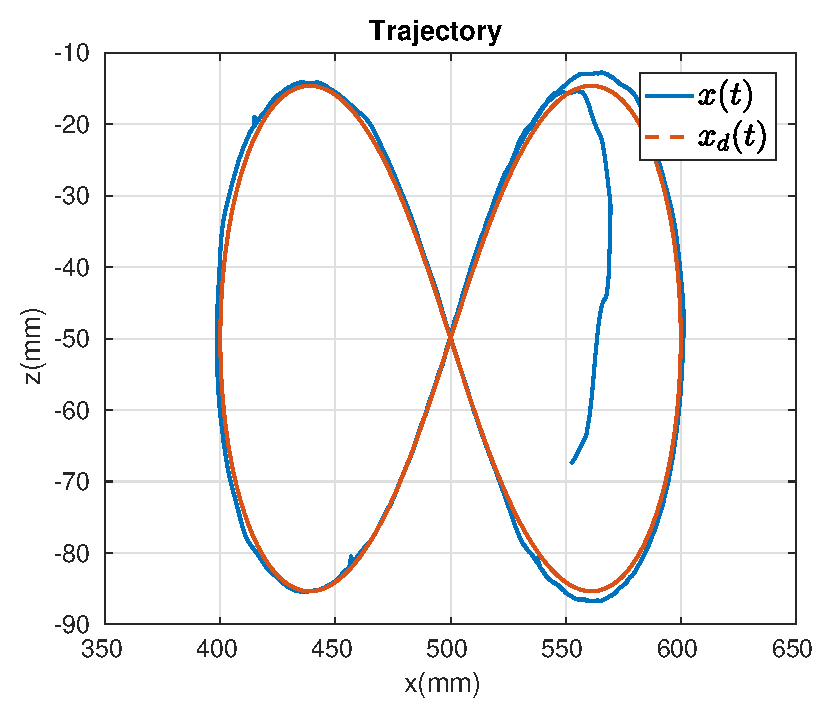
\includegraphics[width=0.5\linewidth]{./img/traj_2_k5/traj.eps}
  \caption{Trajetória 2 no plano x-z para $\bm{K}_t = 5\bm{I}$}
  \label{fig:sub1}
\end{figure}%

\begin{figure}[H]
\centering
\begin{subfigure}{.5\textwidth}
  \centering
  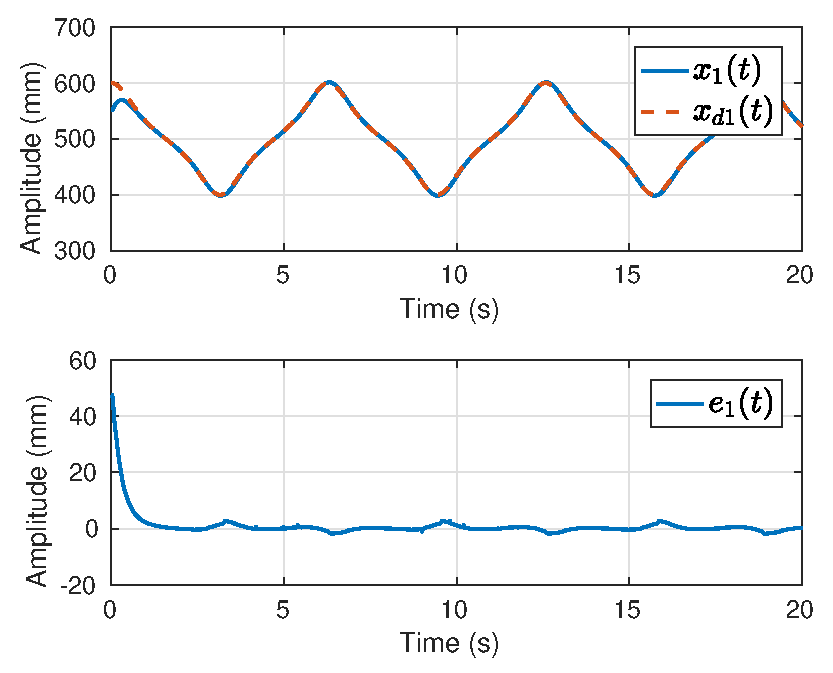
\includegraphics[width=\linewidth]{./img/traj_2_k5/x1.eps}
  \caption{$x_1$, $x_{d1}$ e $e_1$}
  \label{fig:sub1}
\end{subfigure}%
\begin{subfigure}{.5\textwidth}
  \centering
  \includegraphics[width=\linewidth]{./img/traj_2_k5/x2.eps}
  \caption{$x_2$, $x_{d2}$ e $e_2$}
  \label{fig:sub2}
\end{subfigure}
\begin{subfigure}{.5\textwidth}
  \centering
  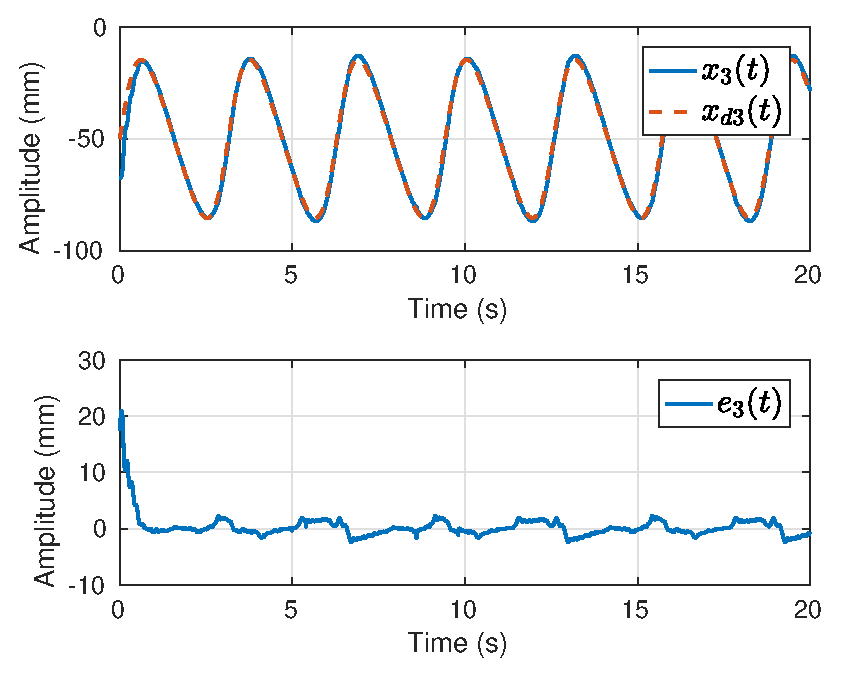
\includegraphics[width=\linewidth]{./img/traj_2_k5/x3.eps}
  \caption{$x_3$, $x_{d3}$ e $e_3$}
  \label{fig:sub1}
\end{subfigure}%
\begin{subfigure}{.5\textwidth}
  \centering
  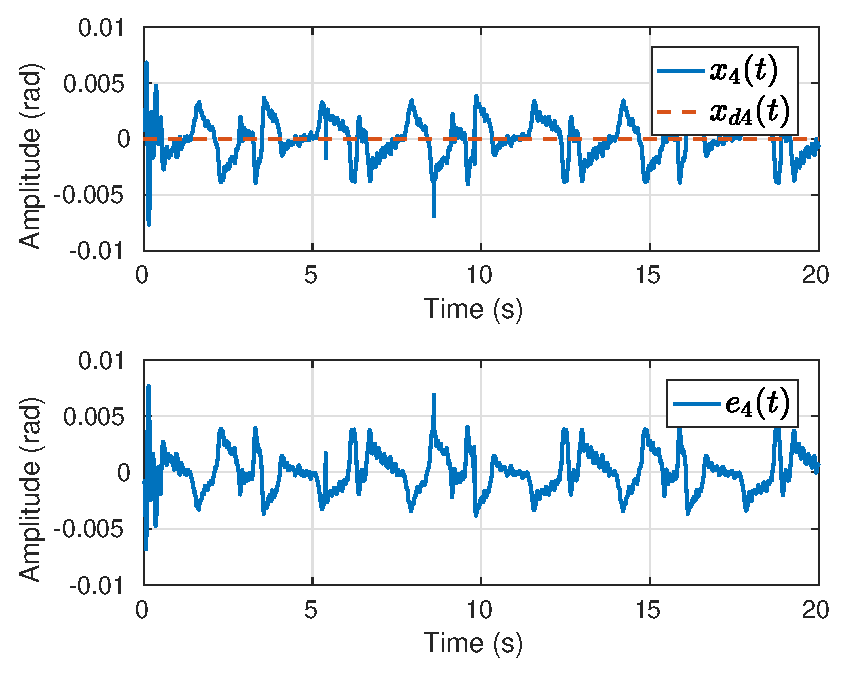
\includegraphics[width=\linewidth]{./img/traj_2_k5/x4.eps}
  \caption{$x_4$, $x_{d4}$ e $e_4$}
  \label{fig:sub2}
\end{subfigure}
\caption{Rastreamento da trajetória 2 para $\bm{K}_t = 5\bm{I}$}
\label{fig:test}
\end{figure}

\begin{figure}[H]
\centering
\begin{subfigure}{.5\textwidth}
  \centering
  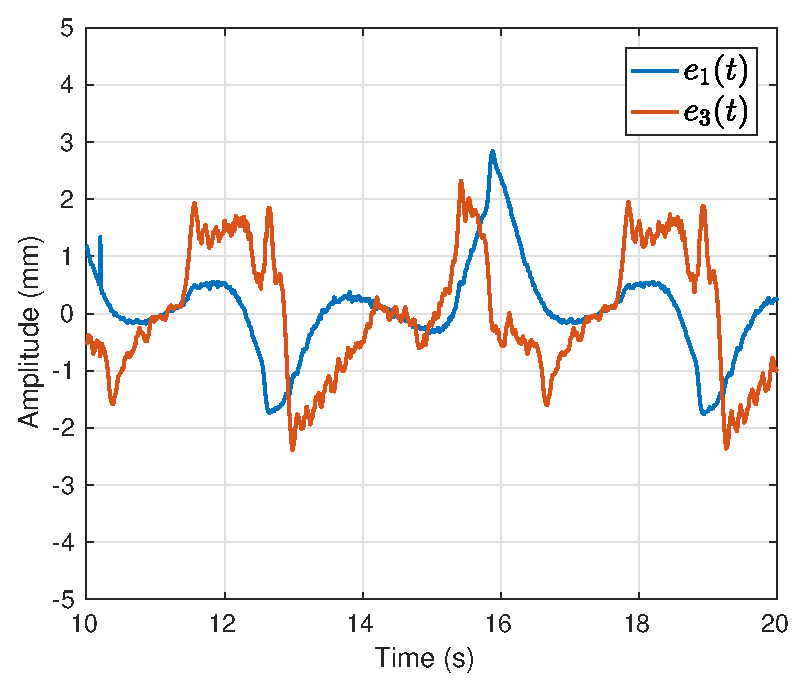
\includegraphics[width=\linewidth]{./img/traj_2_k5/error.eps}
  \caption{$e_1$}
  \label{fig:sub1}
\end{subfigure}%
\begin{subfigure}{.5\textwidth}
  \centering
  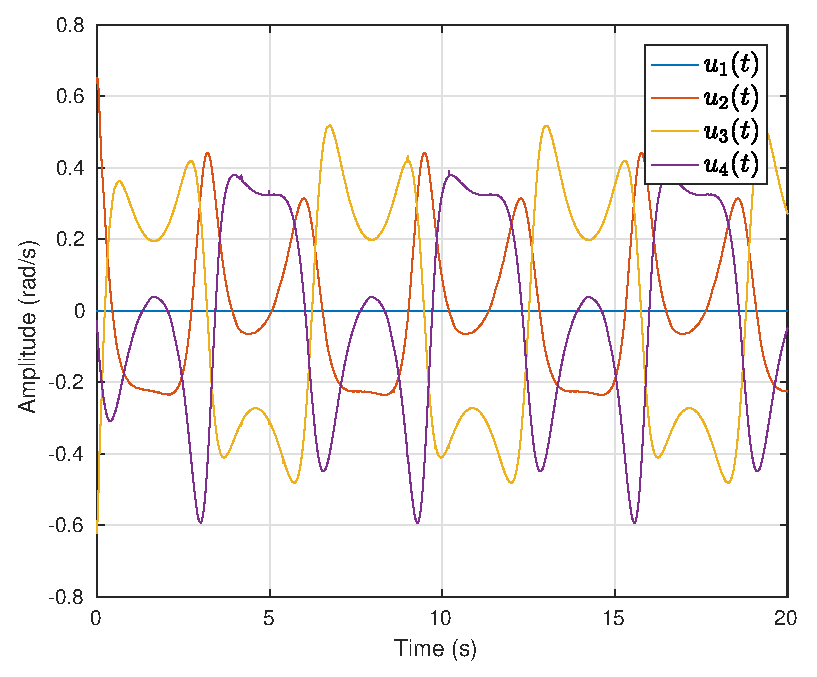
\includegraphics[width=\linewidth]{./img/traj_2_k5/u.eps}
  \caption{$e_3$}
  \label{fig:sub2}
\end{subfigure}
\caption{Trajetória 2: destaque para o erro $e_1$ e $e_3$}
\label{fig:erro_traj}
\end{figure}


\section{Controle de Força}

\subsection{Float}
Neste experimento a referência de força é configurada para zero, logo é possível mover o efetuador aplicando forças sobre ele. O operador tentou traçar um retângulo no plano x-z.

\begin{figure}[H]
\centering
\begin{subfigure}{.5\textwidth}
  \centering
  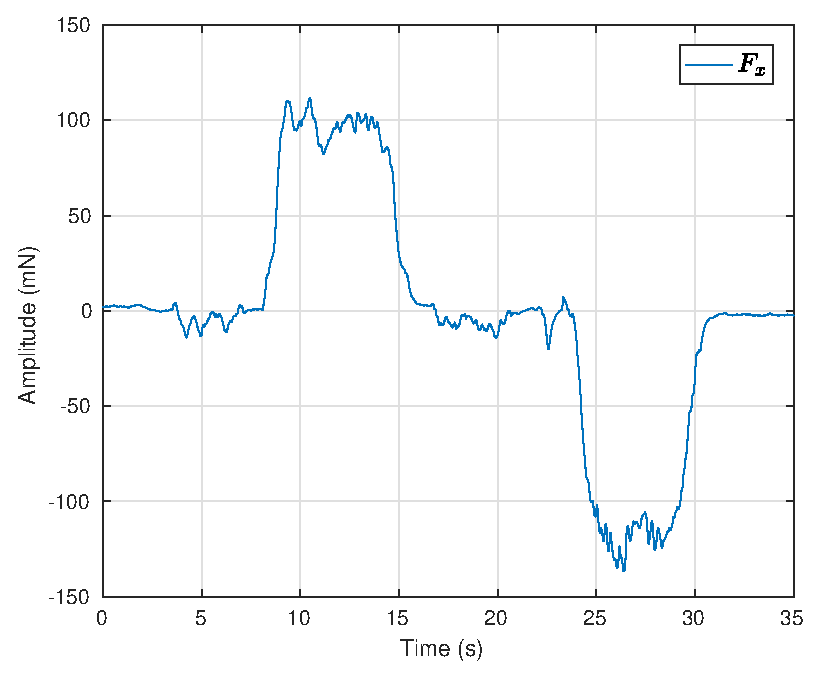
\includegraphics[width=\linewidth]{./img/float2/Fx.eps}
  \caption{$F_x$}
  \label{fig:sub1}
\end{subfigure}%
\begin{subfigure}{.5\textwidth}
  \centering
  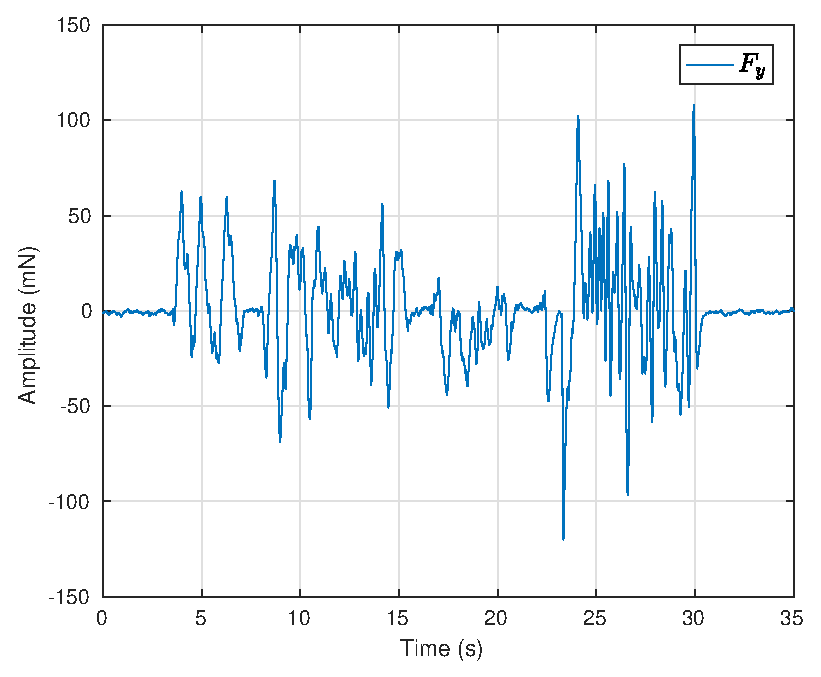
\includegraphics[width=\linewidth]{./img/float2/Fy.eps}
  \caption{$F_y$}
  \label{fig:sub2}	
\end{subfigure}
\begin{subfigure}{.5\textwidth}
  \centering
  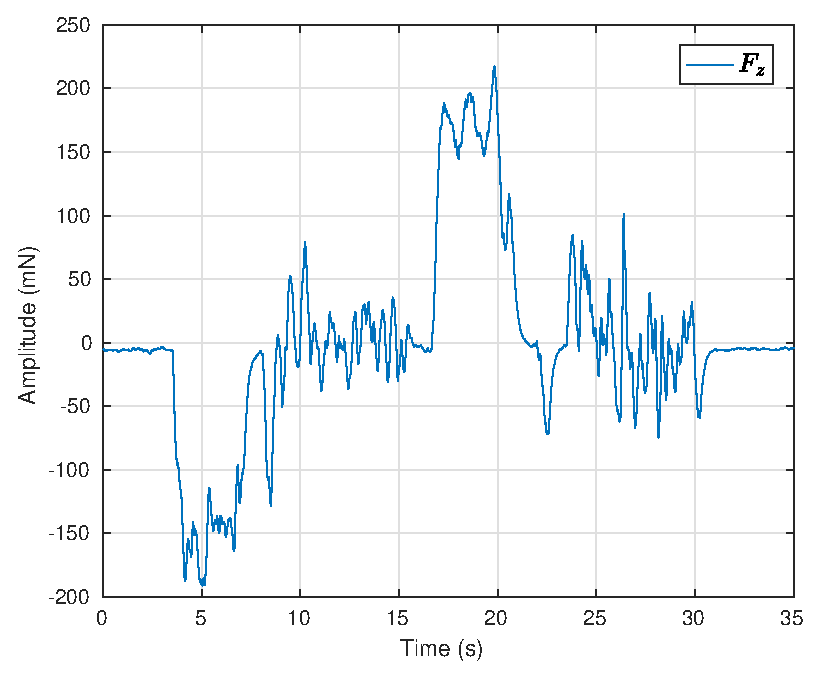
\includegraphics[width=\linewidth]{./img/float2/Fz.eps}
  \caption{$F_z$}
  \label{fig:sub1}
\end{subfigure}%
\begin{subfigure}{.5\textwidth}
  \centering
  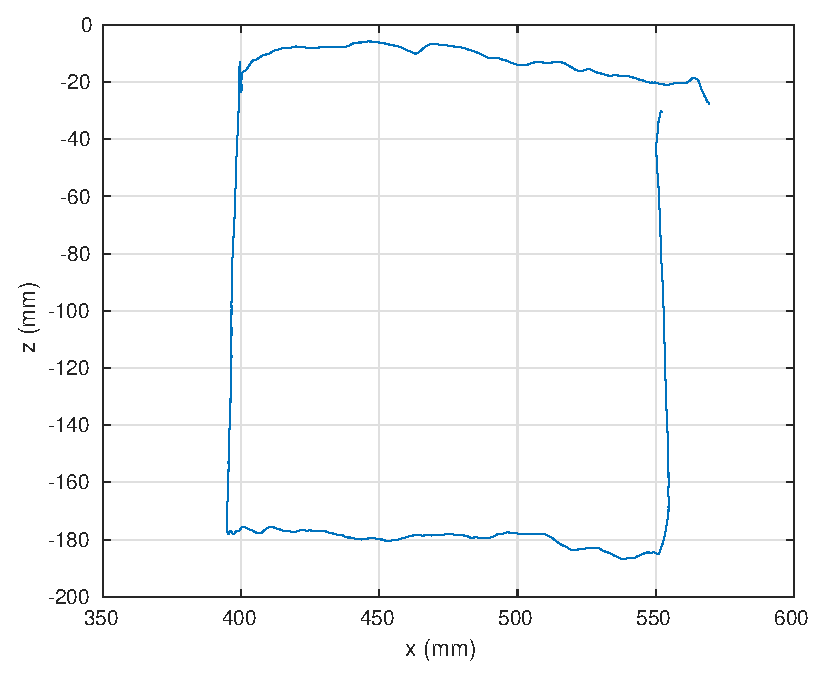
\includegraphics[width=\linewidth]{./img/float2/xz.eps}
  \caption{Plano $xz$}
  \label{fig:sub2}
\end{subfigure}
\caption{Controle de Força: Float}
\label{fig:test}
\end{figure}

\subsection{Approach}

Foi aplicado o controle de força somente na direção de \textit{approach}, sobre uma placa de poliestireno utilizando ganho do controlador PI de $k_p = 2$ e $k_i = 0.05$. A referência de força é de $F_{xd} = 1000 mN$.

 \begin{figure}[H]
  \centering
  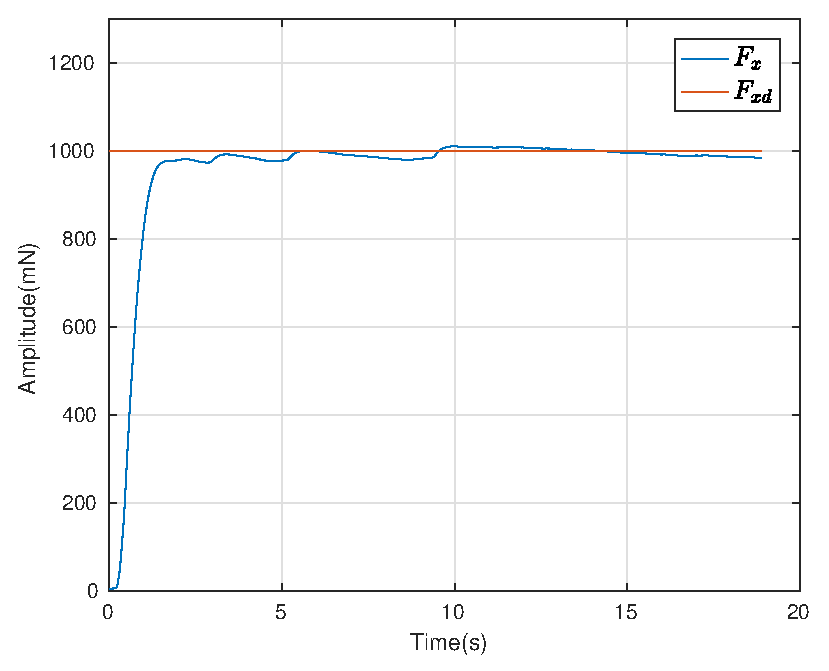
\includegraphics[width=0.5\linewidth]{./img/force1000_kp2_ki005/Fx.eps}
  \caption{Controle de força: Approach $Fx$}
  \label{fig:sub2}
\end{figure}